%\documentclass{cwpreport} % for review/editing/polishing
%\linespread{1.5}           % for review/editing/polishing
\documentclass[onecolumn]{cwpreport} % for final draft

\usepackage{tikz}
\usetikzlibrary{arrows.meta, positioning, fit, backgrounds, calc}

% ── Colors ──────────────────────────────────────────────────────────
\definecolor{topcolor}   {RGB}{255, 255, 255}
\definecolor{motorcolor} {RGB}{255, 255, 255}
\definecolor{ctrlcolor}  {RGB}{255, 255, 255}
\definecolor{comcolor}   {RGB}{255, 255, 255}
\definecolor{sensorcolor}{RGB}{255, 255, 255}
\definecolor{pccolor}    {RGB}{255, 255, 255}


% Packages used by default CWP reports built by M8R
\usepackage{times,natbib,amsmath,graphicx,color,amssymb,amsbsy,lineno,setspace,algorithm2e,lipsum}

% ── Styles ──────────────────────────────────────────────────────────
\tikzset{
	baseblock/.style={
		rectangle, rounded corners=5pt,
		minimum width=2.4cm, minimum height=0.9cm,
		align=center, font=\small\bfseries,
		draw=black!60, line width=0.8pt
	},
	arrow/.style={
		-{Stealth[length=6pt]}, line width=1.2pt, color=black!65
	},
	dblarrow/.style={
		{Stealth[length=6pt]}-{Stealth[length=6pt]},
		line width=1.2pt, color=black!65
	},
	dasharrow/.style={
		-{Stealth[length=6pt]}, dashed, line width=1.2pt, color=black!65
	},
	groupbox/.style={
		draw=black!35, dashed, rounded corners=8pt,
		line width=1pt, fill=gray!7
	}
}

% Specific paper formatting for CWP report
\setlength{\paperwidth}{8.5in}
\setlength{\paperheight}{11.0in}
\setlength{\topmargin}{-0.25in}
\setlength{\textheight}{8.75in}
\setlength{\textwidth}{6.5in}
\setlength{\oddsidemargin}{+.015625in}
\setlength{\evensidemargin}{+.015625in}

% Final draft only
\title[Short Title]{Orca ROV Control System} 
% for editing/reviewing
%\title{Measuring wave propagation through an open-pit mine using stereo videos} 
%\righthead{training data}
%\lefthead{Rapstine & Sava}

% Final draft only
\author[]{Islam Tarek
\\
Capital university, Faculty of engineering in Helwan.\\ islam.my01@gmail.com} 
%
%\author{Thomas Rapstine, Paul Sava, Ashley Grant, \& Jeff Shragge}
\begin{document}

\maketitle

% Uncomment for final draft only
%\setcounter{page}{1}
%\journal{CWP-999}

%% ------------------------------------------------------------
\begin{abstract}
Control is everything to us as humans. The difference between humans and any other creature is our ability to control anything and harness it to do what we want. And the greater a nation's ability to control, the more it dominates other nations. This article presents one way in which a human (me) controls a machine that understands only the language of electrical energy.
\end{abstract}
%% ------------------------------------------------------------

%% ------------------------------------------------------------
\section{Introduction}
The general idea behind the control here is to steer the ROV using commands received from the computer vision model displayed on the front camera. The brain of our ROV; the ESP32-s3 Figure[\ref{fig:esp32-s3-devkitc-1-v1}] receives the information it will use for steering from two sources:
\begin{enumerate}
	\item The laptop containing the computer vision model connected to the camera.
	\item The sensors installed on the ROV.
\end{enumerate}
The microcontroller uses these two sources to calculate the amount of power each motor will need to perform the required task, which is to steer the ROV through the water, capture the required particles, and maintain its balance during the task.

The control system was built using a printed circuit board (PCB) with a set of sensors for acceleration, gyroscope, temperature, and water pressure. The PCB is connected to drivers suitable for the motors used, which receive their commands directly from the ESP32-S3 DevKit to drive the motors.
\begin{figure}
	\centering
	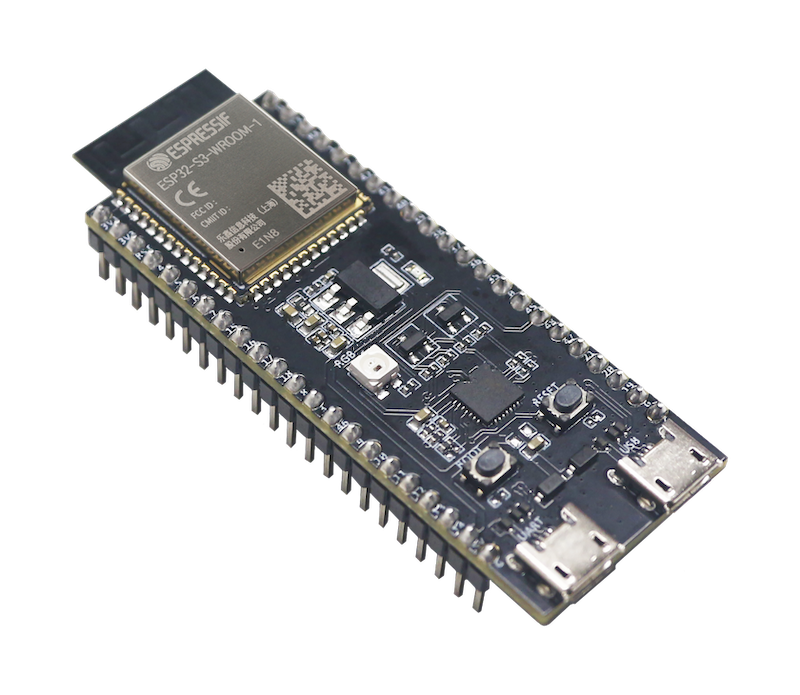
\includegraphics[width=0.5\linewidth]{Fig/esp32-s3-devkitc-1-v1.1-isometric}
	\caption{esp32-s3 DevKit}
	\label{fig:esp32-s3-devkitc-1-v1}
\end{figure}

\section{Overview}
As seen in Figure[\ref{daia}], the power supply provides the ESP32, ESP cam, and motor drivers with the power necessary for their operation.

The ESP32 is connected to control the motor drivers, which are in turn connected to the motors that drive the pumps and the actuator layer. The ESP32 also connects to the sensors to receive the data needed to process the motion commands sent to the motor drivers. The ESP32 also connects to the USB hub to send sensor data and receive motion commands. The ESP cam, which transmits live video, is also connected to the USB hub.

The USB hub is connected to a USB/CAT5 converter so that data can be transferred via a CAT5 cable, chosen for its durability and ability to transmit data over relatively long distances without issues.

The other end of the cable is connected to a CAT/USB converter to the USB 3.0 port on the computer housing the computer vision system.


\begin{figure}
	\centering
\begin{tikzpicture}[node distance=1.1cm and 2.2cm]
	
	%% ═══════════════════════════════
	%%  ROW 0 — Pumps + Arm
	%%  محور X ثابت: pump1=0, pump2=3.8cm, arm=7.6cm
	%% ═══════════════════════════════
	\node[baseblock, fill=topcolor] (pump1) at (0,0)     {Pump 1};
	\node[baseblock, fill=topcolor] (pump2) at (3.8,0)   {Pump 2};
	\node[baseblock, fill=topcolor] (arm)   at (7.6,0)   {Arm};
	
	%% ═══════════════════════════════
	%%  ROW 1 — Motors
	%% ═══════════════════════════════
	\node[baseblock, fill=motorcolor] (m1) at (0,-1.8)   {Motor 1};
	\node[baseblock, fill=motorcolor] (m2) at (3.8,-1.8) {Motor 2};
	\node[baseblock, fill=motorcolor] (mn) at (7.6,-1.8) {Motor n};
	\node[font=\large\bfseries]    (dots) at (5.7,-0.9)  {.....};
	
	%% ═══════════════════════════════
	%%  ROW 2 — Motors Drivers  (مركز عند x=3.8)
	%% ═══════════════════════════════
	\node[baseblock, fill=ctrlcolor,
	minimum width=8.0cm,
	minimum height=1.0cm] (drivers) at (3.8,-3.6) {Motors Drivers};
	
	%% Power Supply — يسار الـ drivers
	\node[baseblock, fill=comcolor,
	minimum width=2.0cm,
	minimum height=1.5cm] (psu) at (-2.0,-3.6) {Power\\Supply};
	
	%% ═══════════════════════════════
	%%  ROW 3 — ESP32-S3  (مركز عند x=3.8)
	%% ═══════════════════════════════
	\node[baseblock, fill=ctrlcolor,
	minimum width=2.8cm] (esp) at (3.8,-5.4) {ESP32-S3};
	
	\node[baseblock, fill=sensorcolor,
	minimum width=2.4cm] (sensors) at (7.2,-5.4) {Sensors};
	
	%% ═══════════════════════════════
	%%  ROW 4 — ESP-CAM (خارج الـ box يسار) و USB HUB (داخل الـ box)
	%% ═══════════════════════════════
	\node[baseblock, fill=comcolor] (espcam) at (-2.0,-7.2) {ESP-CAM};
	\node[baseblock, fill=comcolor] (usbhub) at (3.8,-7.2)  {USB HUB};
	
	%% ═══════════════════════════════
	%%  ROW 5-7 — Communication chain  (محاذاة مع USB HUB عند x=6.2)
	%% ═══════════════════════════════
	\node[baseblock, fill=comcolor,
	minimum width=2.8cm] (usb2cat5) at (3.8,-8.9)  {USB--CAT5\\Converter};
	
	\node[baseblock, fill=comcolor,
	minimum width=2.8cm] (cat5)     at (3.8,-10.5) {CAT5 Cable};
	
	\node[baseblock, fill=comcolor,
	minimum width=2.8cm] (cat52usb) at (3.8,-12.1) {CAT5--USB\\Converter};
	
	\node[baseblock, fill=pccolor,
	minimum width=2.4cm] (computer) at (7.2,-12.1) {Computer};
	
	%% ═══════════════════════════════
	%%  ARROWS
	%% ═══════════════════════════════
	
	% Motors → Actuators
	\draw[arrow] (m1) -- (pump1);
	\draw[arrow] (m2) -- (pump2);
	\draw[arrow] (mn) -- (arm);
	
	% Drivers → Motors
	\draw[arrow] (drivers.north -| m1) -- (m1.south);
	\draw[arrow] (drivers.north -| m2) -- (m2.south);
	\draw[arrow] (drivers.north -| mn) -- (mn.south);
	
	% Power Supply → ESP32 (من الجانب مع الـ Drivers)
	\draw[arrow] (psu.east) -- (drivers.west);
	\draw[arrow] (psu.south) -- ++(0,-1.0) -- (esp.west);
	
	% Power Supply → ESP-CAM (عمودي مستقيم)
	\draw[arrow] (psu.south) -- (espcam.north);
	
	% Drivers ↔ ESP32 (dashed)
	\draw[arrow] (esp.north) -- (drivers.south);
	
	% Sensors → ESP32
	\draw[arrow] (sensors.west) -- (esp.east);
	
	% ESP32 → USB HUB
	\draw[dblarrow] (esp.south) -- ++(0,-0.5) -| (usbhub.north);
	
	% Power Supply → ESP-CAM
	\draw[arrow] (psu.south) -- (espcam.north);
	
	% ESP-CAM ↔ USB HUB
	\draw[dblarrow] (espcam.east) -- (usbhub.west);
	
	% Communication chain
	\draw[dblarrow] (usbhub)   -- (usb2cat5);
	\draw[dblarrow] (usb2cat5) -- (cat5);
	\draw[dblarrow] (cat5)     -- (cat52usb);
	
	% CAT5-USB ↔ Computer
	\draw[dblarrow] (cat52usb.east) -- (computer.west);
	
	%% ═══════════════════════════════
	%%  GROUP BOXES
	%% ═══════════════════════════════
	\begin{scope}[on background layer]
		
		\node[groupbox,
		fit=(pump1)(pump2)(arm)(m1)(m2)(mn)(dots),
		inner sep=10pt,
		label={[font=\small\itshape, text=black!50]above:Actuator Layer}] {};
		
		\node[groupbox,
		fit=(usbhub)(usb2cat5)(cat5)(cat52usb),
		inner sep=14pt,
		label={[font=\small\itshape, text=black!50]below left:Communication Channel}] {};
	\end{scope}
\end{tikzpicture}
\label{daia}
\caption{Control system diagram}
\end{figure}

\newpage
\section{PCB and circuit diagram}
\begin{figure}
	\centering
	\includegraphics[width=0.9\linewidth]{"Fig/Pasted image (2)"}
	\caption{}
	\label{fig:pasted-image-2}
\end{figure}
\begin{figure}
	\centering
	\includegraphics[width=0.9\linewidth]{"Fig/image"}
	\caption{}
	\label{fig:pasted--2}
\end{figure}

\newpage
\begin{figure}
	\centering
	\begin{tikzpicture}[node distance=1.1cm and 2.2cm]
		
		
		%% ═══════════════════════════════
		%%  ROW 2 — Motors Drivers  (مركز عند x=3.8)
		%% ═══════════════════════════════
		\node[baseblock, fill=ctrlcolor,
		minimum width=8.0cm,
		minimum height=1.0cm] (drivers) at (3.8,-3.6) {Motors Drivers};
		
		%% Power Supply — يسار الـ drivers
		\node[baseblock, fill=comcolor,
		minimum width=2.0cm,
		minimum height=1.5cm] (psu) at (-2.0,-3.6) {Power\\Supply};
		
		%% ═══════════════════════════════
		%%  ROW 3 — ESP32-S3  (مركز عند x=3.8)
		%% ═══════════════════════════════
		\node[baseblock, fill=ctrlcolor,
		minimum width=2.8cm] (esp) at (3.8,-5.4) {ESP32-S3};

		
		%% ═══════════════════════════════
		%%  ROW 4 — ESP-CAM (خارج الـ box يسار) و USB HUB (داخل الـ box)
		%% ═══════════════════════════════
		\node[baseblock, fill=comcolor] (espcam) at (-2.0,-7.2) {ESP-CAM};
		

	
		% Power Supply → ESP32 (من الجانب مع الـ Drivers)
		\draw[arrow] (psu.east) -- (drivers.west);
		\draw[arrow] (psu.south) -- ++(0,-1.0) -- (esp.west);
		
		% Power Supply → ESP-CAM (عمودي مستقيم)
		\draw[arrow] (psu.south) -- (espcam.north);
		
		
		
		% Power Supply → ESP-CAM
		\draw[arrow] (psu.south) -- (espcam.north);

	\end{tikzpicture}
	\label{power}
	\caption{Control system diagram}
\end{figure}

\begin{figure}
	\centering
	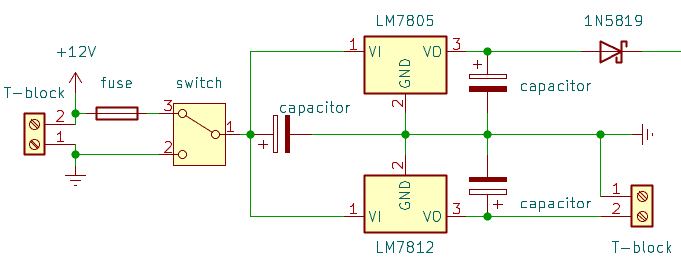
\includegraphics[width=0.7\linewidth]{Fig/power}
	\caption{Voltage regulation network}
	\label{fig:power}
\end{figure}

\section{Power supply}
The ESP32 is an excellent microcontroller (for its class) due to its fast clock and relatively large internal memory. However, it suffers from a problem that makes many people avoid it. Its main issue is its sensitivity to power voltage. If a certain voltage is exceeded or there is a sudden change in voltage, it will be completely damaged. Therefore, we must first ensure a stable DC voltage.

The ROV's power supply is a stable 24V DC. To reduce this voltage to the value required by the ESP32, we will use an electronic component called the LM7805, which is a voltage regulator. Its function is to reduce the voltage to 5V to supply the ESP32.

This electronic component is connected to a capacitor at both the input and output to ensure voltage stability. A Zener diode is connected at the end of the circuit directly to the ESP32's power supply port to prevent any reverse current Figure[\ref{fig:power}].

I connected another Voltage regulation circuit to make another branch for the motor drivers which needs a 12 volts of DC voltage. the whole circuit called a voltage regulation network.


\newpage

\section{Actuators}
The actuator network layer is one of the most important layers, and the entire system was built around it. As its name suggests, it's responsible for the actual, real-world action. The entire system is meaningless without it, so I made sure to select the appropriate components.

As shown in Figure[\ref{act}], the ESP connects to the drivers in Figure[\ref{fig:a4988}] to control the motors. A set of ZK-BM1s (on the right) is used to control the DC motors connected to the pumps. One of these can control two motors simultaneously. The A4988 is used to control the stepper motor connected to the arm.


\begin{figure}
	\centering
	\begin{tikzpicture}[node distance=1.1cm and 2.2cm]
		
		%% ═══════════════════════════════
		%%  ROW 0 — Pumps + Arm
		%%  محور X ثابت: pump1=0, pump2=3.8cm, arm=7.6cm
		%% ═══════════════════════════════
		\node[baseblock, fill=topcolor] (pump1) at (0,0)     {Pump 1};
		\node[baseblock, fill=topcolor] (pump2) at (3.8,0)   {Pump 2};
		\node[baseblock, fill=topcolor] (arm)   at (7.6,0)   {Arm};
		
		%% ═══════════════════════════════
		%%  ROW 1 — Motors
		%% ═══════════════════════════════
		\node[baseblock, fill=motorcolor] (m1) at (0,-1.8)   {Motor 1};
		\node[baseblock, fill=motorcolor] (m2) at (3.8,-1.8) {Motor 2};
		\node[baseblock, fill=motorcolor] (mn) at (7.6,-1.8) {Motor n};
		\node[font=\large\bfseries]    (dots) at (5.7,-0.9)  {.....};
		
		%% ═══════════════════════════════
		%%  ROW 2 — Motors Drivers  (مركز عند x=3.8)
		%% ═══════════════════════════════
		\node[baseblock, fill=ctrlcolor,
		minimum width=8.0cm,
		minimum height=1.0cm] (drivers) at (3.8,-3.6) {Motors Drivers};
		
		
		%% ═══════════════════════════════
		%%  ROW 3 — ESP32-S3  (مركز عند x=3.8)
		%% ═══════════════════════════════
		\node[baseblock, fill=ctrlcolor,
		minimum width=2.8cm] (esp) at (3.8,-5.4) {ESP32-S3};
		
		
		
		%% ═══════════════════════════════
		%%  ARROWS
		%% ═══════════════════════════════
		
		% Motors → Actuators
		\draw[arrow] (m1) -- (pump1);
		\draw[arrow] (m2) -- (pump2);
		\draw[arrow] (mn) -- (arm);
		
		% Drivers → Motors
		\draw[arrow] (drivers.north -| m1) -- (m1.south);
		\draw[arrow] (drivers.north -| m2) -- (m2.south);
		\draw[arrow] (drivers.north -| mn) -- (mn.south);
		
		% Drivers ↔ ESP32 (dashed)
		\draw[arrow] (esp.north) -- (drivers.south);
		



		
		%% ═══════════════════════════════
		%%  GROUP BOXES
		%% ═══════════════════════════════
		\begin{scope}[on background layer]
			\node[groupbox,
			fit=(pump1)(pump2)(arm)(m1)(m2)(mn)(dots),
			inner sep=10pt,
			label={[font=\small\itshape, text=black!50]above:Actuator Layer}] {};
		\end{scope}
	\end{tikzpicture}
	\label{act}
	\caption{Actuators network diagram}
\end{figure}
\begin{figure}
	\centering
	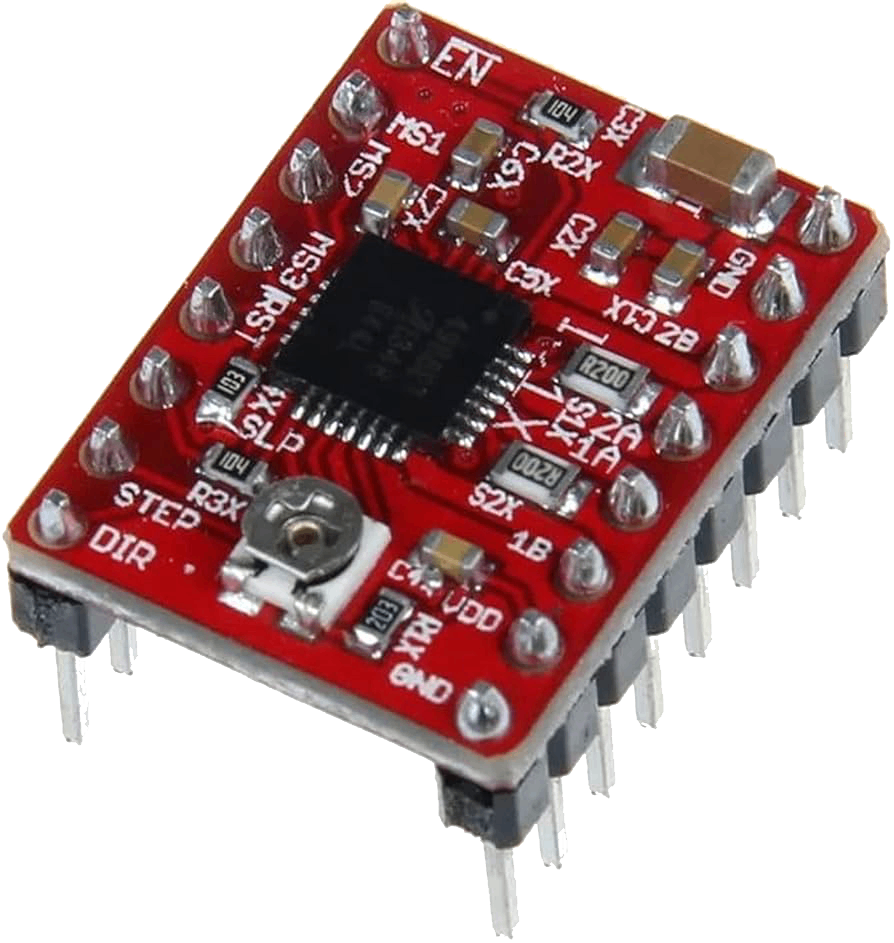
\includegraphics[width=0.3\linewidth]{Fig/A4988}
	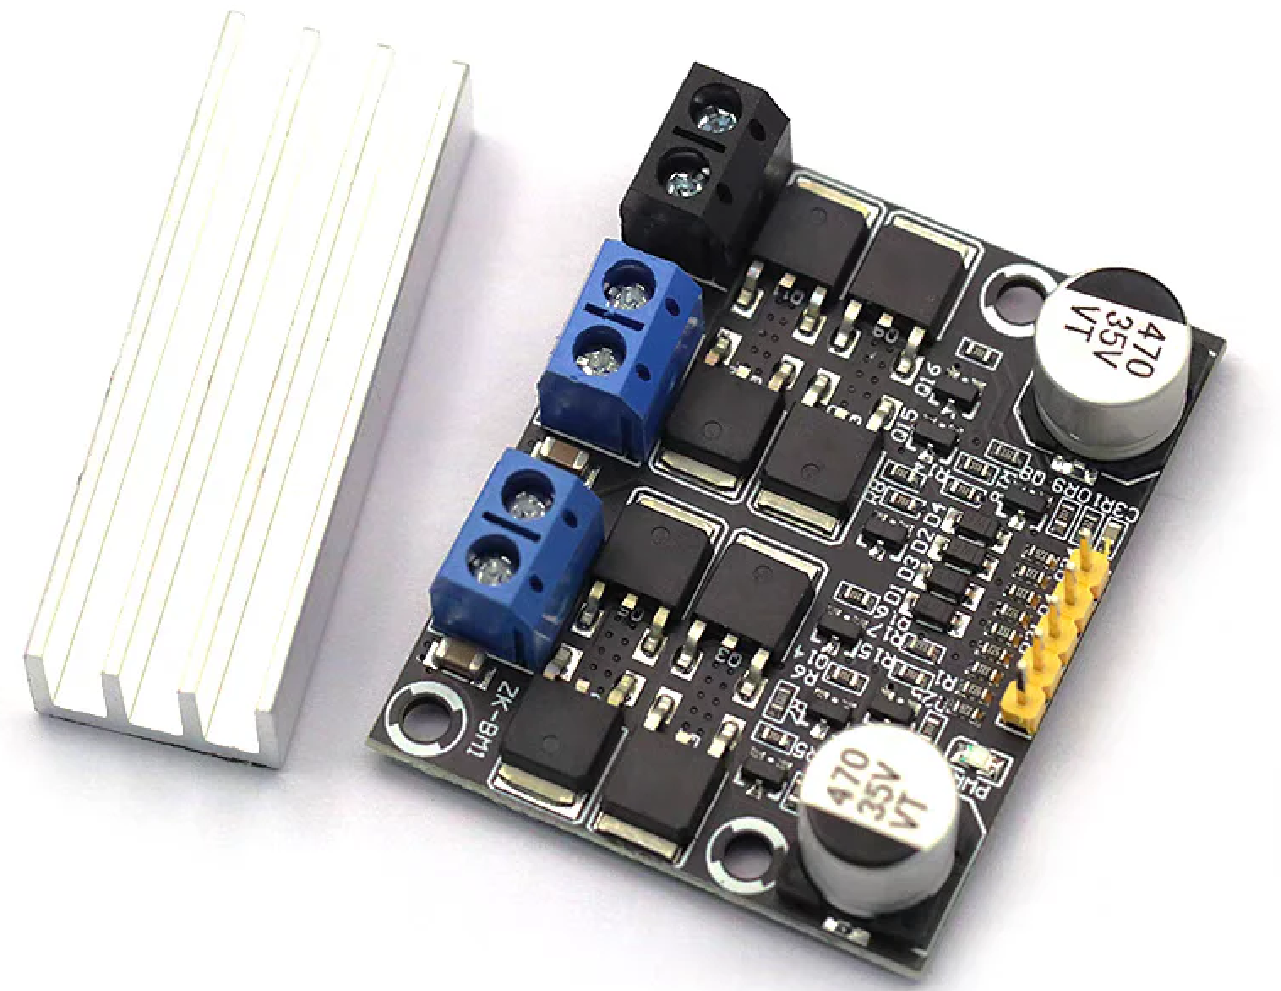
\includegraphics[width=0.45\linewidth]{Fig/Pasted image}
	\caption{Drivers}
	\label{fig:a4988}
\end{figure}

\newpage

\section{Sensors}
Sensors are what allow the ROV to "feel" its surroundings and understand its own movement. Without them, the ROV would be blind and unable to make any decisions.
The ROV uses two types of sensors:
The first type is connected directly to the ESP32-S3. These sensors measure physical conditions in real time — the MPU6050 (Figure~\ref{fig:932}-left) tracks the ROV's orientation and movement, while the GT MS5837 (Figure~\ref{fig:932}-middle) measures water pressure and temperature. The ESP32-S3 reads this data instantly and uses it to make decisions on its own.
The second type is the ESP32-CAM (Figure~\ref{fig:932}-right), which acts as the ROV's eyes. It streams live video through the USB hub directly to the surface computer, so the operator can see exactly what the ROV sees.
\begin{figure}
	\centering
	\begin{tikzpicture}[node distance=1.1cm and 2.2cm]
		%% ═══════════════════════════════
		%%  ROW 3 — ESP32-S3  (مركز عند x=3.8)
		%% ═══════════════════════════════
		\node[baseblock, fill=ctrlcolor,
		minimum width=2.8cm] (esp) at (3.8,-5.4) {ESP32-S3};
		
		\node[baseblock, fill=sensorcolor,
		minimum width=2.4cm] (sensors) at (7.4,-5.4) {Sensors};
		
		%% ═══════════════════════════════
		%%  ROW 4 — ESP-CAM (خارج الـ box يسار) و USB HUB (داخل الـ box)
		%% ═══════════════════════════════
		\node[baseblock, fill=comcolor] (espcam) at (0,-7.2) {ESP-CAM};
		\node[baseblock, fill=comcolor] (usbhub) at (3.8,-7.2)  {USB HUB};
		

		
		%% ═══════════════════════════════
		%%  ARROWS
		%% ═══════════════════════════════

		
		% Sensors → ESP32
		\draw[arrow] (sensors.west) -- (esp.east);
		
		% ESP32 → USB HUB
		\draw[dblarrow] (esp.south) -- ++(0,-0.5) -| (usbhub.north);
		
		% ESP-CAM ↔ USB HUB
		\draw[dblarrow] (espcam.east) -- (usbhub.west);
		
		
	\end{tikzpicture}
	\label{sens}
	\caption{Control system diagram}
\end{figure}

\begin{figure}
	\centering
	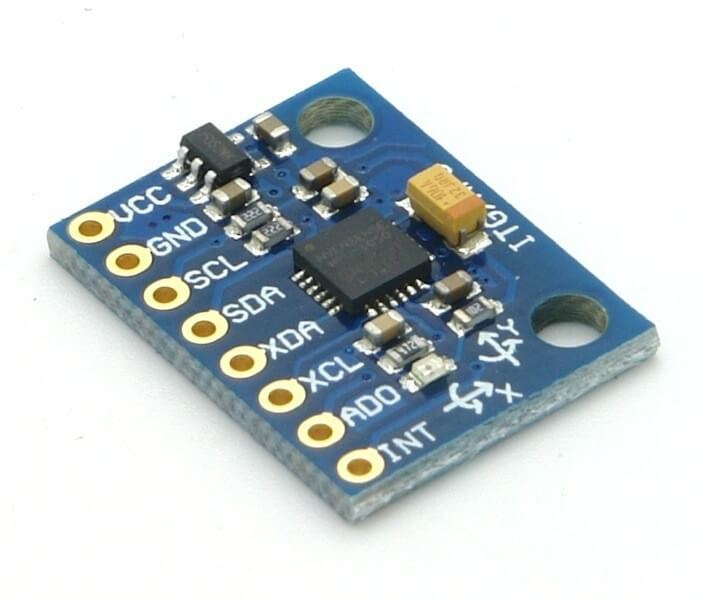
\includegraphics[width=0.29\linewidth]{Fig/932}
	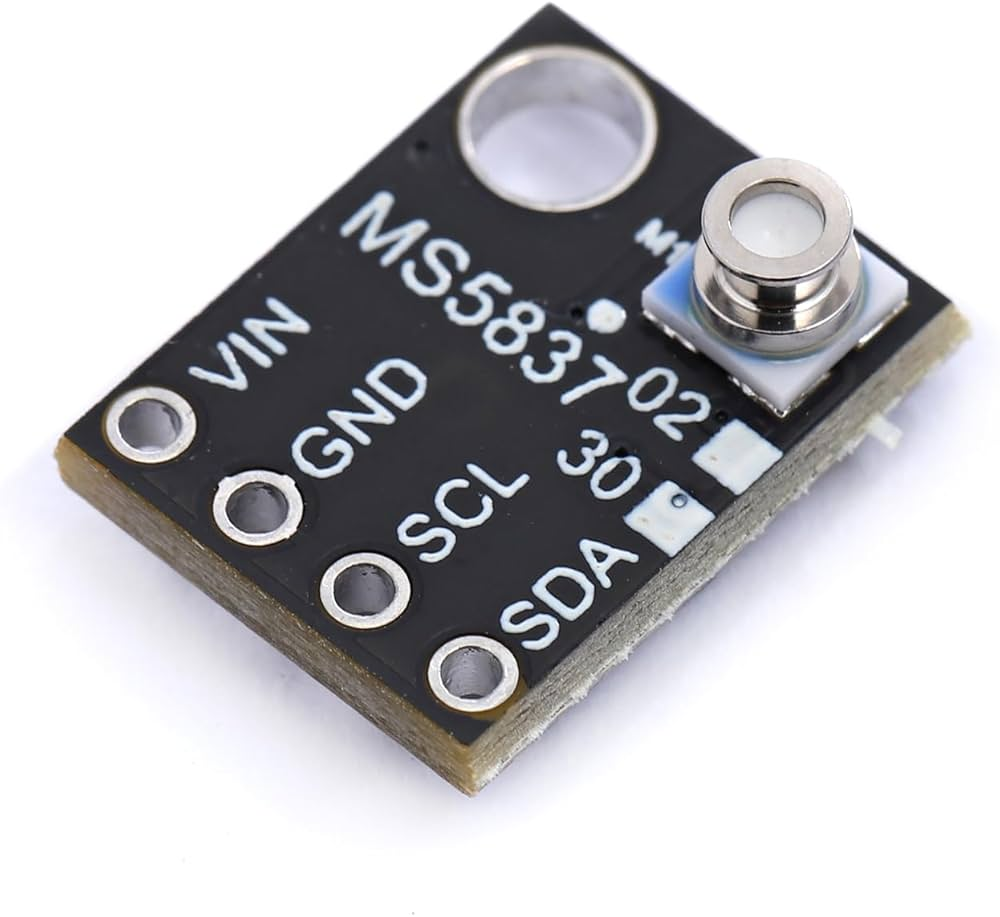
\includegraphics[width=0.29\linewidth]{Fig/5}
	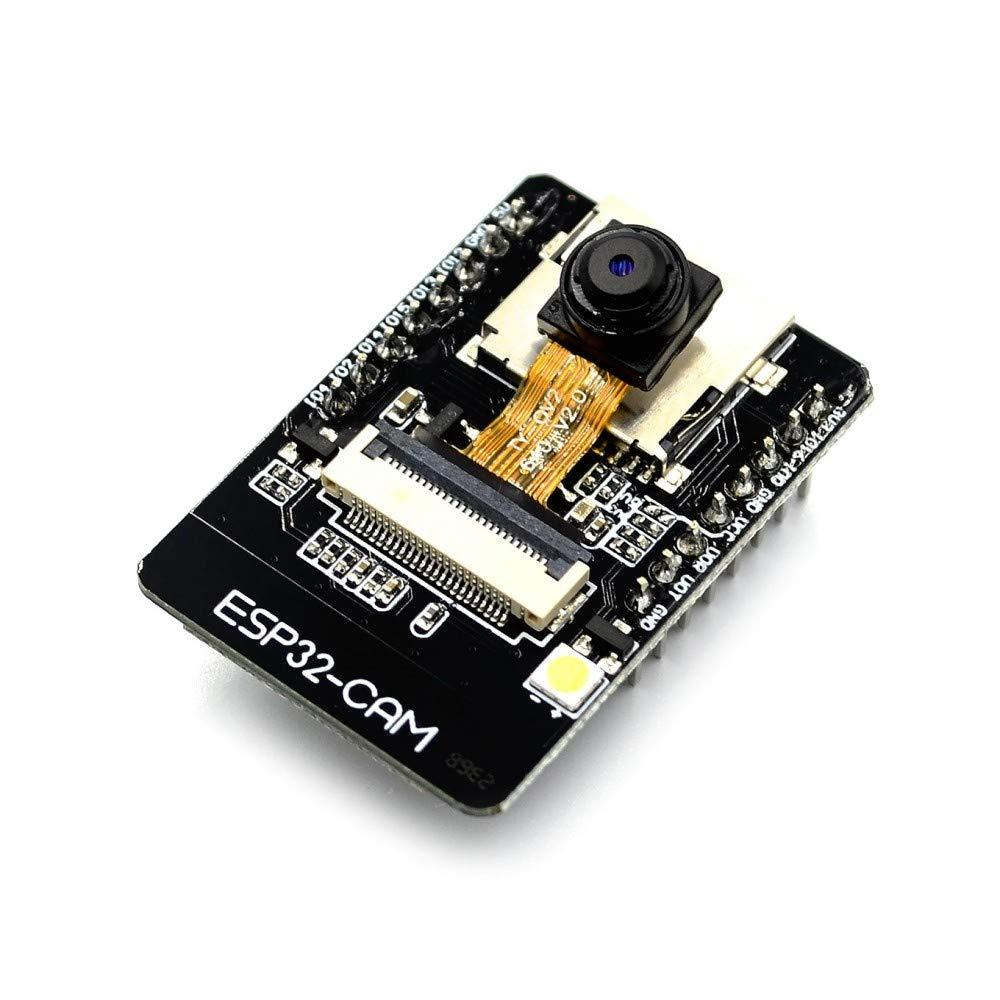
\includegraphics[width=0.4\linewidth]{Fig/FCEU2OXLOMX063A}
	\caption{}
	\label{fig:932}
\end{figure}

\newpage

\section{Communication}
Because the ESP32 cannot process or store computer vision models, we need to connect the ROV to a computer to analyze this information and make decisions for the ROV.

We cannot connect the ESP32-S3 and ESP32 CAM directly via USB due to the limited range of these connections. Therefore, we will use a CAT5 cable to transmit data over the relatively long distance the ROV will be operating at. To do this, we must first connect the ESP32-S3 and ESP32 CAM to a single line using a USB hub. Then, we convert the output of this USB hub using a USB/CAT5 converter to a format that the CAT5 cable can understand for transmission. Finally, we reverse the process using a CAT/USB converter to connect it to the computer.

\begin{figure}
	\centering
	\begin{tikzpicture}[node distance=1.1cm and 2.2cm]
		
		
		%% ═══════════════════════════════
		%%  ROW 3 — ESP32-S3  (مركز عند x=3.8)
		%% ═══════════════════════════════
		\node[baseblock, fill=ctrlcolor,
		minimum width=2.8cm] (esp) at (0,-5.4) {ESP32-S3};
		
		%% ═══════════════════════════════
		%%  ROW 4 — ESP-CAM (خارج الـ box يسار) و USB HUB (داخل الـ box)
		%% ═══════════════════════════════
		\node[baseblock, fill=comcolor] (espcam) at (-5,-7.2) {ESP-CAM};
		\node[baseblock, fill=comcolor] (usbhub) at (0,-7.2)  {USB HUB};
		
		%% ═══════════════════════════════
		%%  ROW 5-7 — Communication chain  (محاذاة مع USB HUB عند x=6.2)
		%% ═══════════════════════════════
		\node[baseblock, fill=comcolor,
		minimum width=2.8cm] (usb2cat5) at (0,-8.9)  {USB--CAT5\\Converter};
		
		\node[baseblock, fill=comcolor,
		minimum width=2.8cm] (cat5)     at (0,-10.5) {CAT5 Cable};
		
		\node[baseblock, fill=comcolor,
		minimum width=2.8cm] (cat52usb) at (0,-12.1) {CAT5--USB\\Converter};
		
		\node[baseblock, fill=pccolor,
		minimum width=2.4cm] (computer) at (5,-12.1) {Computer};
		
		%% ═══════════════════════════════
		%%  ARROWS
		%% ═══════════════════════════════
		
		% ESP32 → USB HUB
		\draw[dblarrow] (esp.south) -- ++(0,-0.5) -| (usbhub.north);
		
		% ESP-CAM ↔ USB HUB
		\draw[dblarrow] (espcam.east) -- (usbhub.west);
		
		% Communication chain
		\draw[dblarrow] (usbhub)   -- (usb2cat5);
		\draw[dblarrow] (usb2cat5) -- (cat5);
		\draw[dblarrow] (cat5)     -- (cat52usb);
		
		% CAT5-USB ↔ Computer
		\draw[dblarrow] (cat52usb.east) -- (computer.west);
		
		%% ═══════════════════════════════
		%%  GROUP BOXES
		%% ═══════════════════════════════
		\begin{scope}[on background layer]
			\node[groupbox,
			fit=(usbhub)(usb2cat5)(cat5)(cat52usb),
			inner sep=14pt,
			label={[font=\small\itshape, text=black!50]below left:Communication Channel}] {};
		\end{scope}
	\end{tikzpicture}
	\label{comm}
	\caption{Control system diagram}
\end{figure}
%% ------------------------------------------------------------

%% -----------------
\end{document}